\begin{frame}[fragile]{C6-FT-LLL (HR1N unfolded in all protomers)}
    \begin{center}
        \begin{minipage}{0.47\textwidth}
            \begin{center}
                gp120 alignment\\
                \includegraphics[width=\textwidth]{/home/cfa/research/hiv/trifppr/class6/C6_FT_LLL/rotation-matrices-gp120.png}
            \end{center}
        \end{minipage}
        \begin{minipage}{0.47\textwidth}
            \begin{center}
                gp41 alignment\\
                \includegraphics[width=\textwidth]{/home/cfa/research/hiv/trifppr/class6/C6_FT_LLL/rotation-matrices-gp41.png}
            \end{center}
        \end{minipage}

        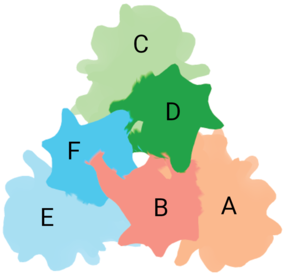
\includegraphics[width=0.19\textwidth]{trimer_paint_bottom_sodroski_smol.png}
        \includegraphics[width=0.19\textwidth]{/home/cfa/research/hiv/trifppr/class6/C6_FT_LLL/images/bottom-view.00000.png}
        \includegraphics[width=0.19\textwidth]{/home/cfa/research/hiv/trifppr/class6/C6_FT_LLL/images/bottom-view.00033.png}
        \includegraphics[width=0.19\textwidth]{/home/cfa/research/hiv/trifppr/class6/C6_FT_LLL/images/bottom-view.00067.png}
        \includegraphics[width=0.19\textwidth]{/home/cfa/research/hiv/trifppr/class6/C6_FT_LLL/images/bottom-view.00099.png}

        Protomer 1 MPER remains relatively stable
    \end{center}
\end{frame}

